\documentclass[12pt]{report}

\def\magyarOptions{defaults=hu-min}
\usepackage[magyar]{babel}
\usepackage[utf8]{inputenc}
\usepackage{t1enc}

\usepackage{times}

\usepackage{amsmath}
\usepackage{amssymb}
\usepackage{amsthm}

\usepackage{enumitem}
\usepackage{fancyhdr}
\usepackage{graphicx}
\usepackage{hyperref}
\usepackage{verbatim}
\usepackage{xcolor}

% Margins
\hoffset -1in
\voffset -1in
\oddsidemargin 35mm
\textwidth 150mm
\topmargin 15mm
\headheight 10mm
\headsep 5mm
\textheight 237mm

% URL style
\hypersetup{
    colorlinks=false, % Disable colorlinks for not coloring table of contents
    unicode=true,
}

\let\orighref\href
\renewcommand{\href}[2]{%
    \orighref{#1}{\textcolor{blue}{\texttt{#2}}}
}

\let\origurl\url
\renewcommand{\url}[1]{%
    \textcolor{blue}{\origurl{#1}}
}

\newcommand{\todo}[1]{%
    \textcolor{red}{\textbf{TODO}}\footnote{\textcolor{red}{\textbf{TODO:} #1}}
}

\newcommand{\fixme}[1]{%
    \textcolor{red}{\textbf{FIXME}}\footnote{\textcolor{red}{\textbf{FIXME:} #1}}
}

\setdescription{
    style=standard,
    align=right,
    itemindent=1cm,
    labelwidth=1cm,
    leftmargin=1cm,
    before={\renewcommand\makelabel[1]{\bfseries ########1:}},
    %font=\sffamily\bfseries,
}

\hyphenation{QtWebEngine QtWebKit WebKit Chromium Content Apple Google Quick Widget}

\def\title{A QtWebEngine bővítése és bemutatása saját böngészőalkalmazás segítségével}

\begin{document}

% EMPTY PAGE STYLE
\fancypagestyle{plain}{
    \fancyhf{}
    \fancyfoot[R]{\thepage}
    \renewcommand{\headrulewidth}{0pt}
}

% FOOTER & HEADER
\pagestyle{fancy}
\fancyhf{}
\fancyhead[L]{\title}
\fancyfoot[R]{\thepage}
%\fancyfoot[C]{\thepage}

%%% TITLE PAGE %%%
\thispagestyle{empty}
\begin{center}
    \vspace*{1cm}
    {\Large\textbf{Szegedi Tudományegyetem}}

    \vspace{0.5cm}
    {\Large\textbf{Informatikai Tanszékcsoport}}

    \vspace{3.8cm}
    {\LARGE\textbf{\title}}

    \vspace{3.6cm}
    {\Large Diplomamunka}

    \vspace{4cm}
    \begin{large}
        \begin{tabular}{c@{\hspace{4cm}}c}
            \emph{Készítette:}      & \emph{Témavezető:}        \\
            \textbf{Varga Péter}    & \textbf{Dr. Kiss Ákos}    \\
            programtervező          & egyetemi adjunktus        \\
            informatikus szakos     &                           \\
            hallgató                &
        \end{tabular}
    \end{large}

    \vspace*{2.3cm}
    \begin{Large}
        Szeged

        \vspace{2mm}
        2016
    \end{Large}
\end{center}


%%% TABLE OF CONTENTS %%%
\tableofcontents

%%% PROLOGUE %%%

\chapter*{Feladatkiírás}
\addcontentsline{toc}{section}{Feladatkiírás}

\noindent
A QtWebEngine bővítése úgy, hogy a QtWebKit-et használó fejlesztők könnyen portolhassák
a projektjüket QtWebEngine-re.
Továbbá, olyan új funkciók megvalósítása is fontos, amelyek hozzásegítik a
QtWebEngine-t, hogy lépést tartson a fejlődő web technológiákkal (pl. HTML5).
Az újonnan implementált funkciókat tesztelni kell.

\bigskip
\noindent
A tesztelésre lehetőséget nyújt a Qt \texttt{auto test}
keretrendszere, viszont bizonyos funkciók nem tesztelhetőek megfelelően \texttt{auto}
tesztekkel, továbbá nem biztosítható teljes lefedettség. A probléma kiküszöbölésére
példa alkalmazás(ok) implementálására van szükség, amelyet a fejlesztő használhat
``manuális'' tesztelésre, hibakeresésre, továbbá annak forráskódja a funkciók
dokumentálására, bemutatására is felhasználható.

\bigskip
\noindent
A fejlesztés során az alábbi szempontokat kell figyelembe venni:
\begin{itemize}
    \item Bináris kompatibilitás megtartása korábbi QtWebEngine verziókkal:
        publikus API-ban a változtatások számát minimalizálni kell,
        meglévő API-t (függvény, property, signal, stb.) módosítani vagy eltávolítani
        nem lehet.
    \item Törekvés kompatibilitásra a QtWebKit-el.
        A QtWebEngine-hez adott új API-k ne térjenek el (névben, paraméterezésben, stb.)
        az eredeti QtWebKit API-tól, hacsak ezt az új funkcionalitás bővítése nem indokolja.
    \item Törekedni kell arra, hogy a Quick és Widget API hasonlítson egymásra,
        amennyire csak lehet.
    \item Az új funkcionalitásokhoz \texttt{auto} tesztet kell készíteni,
        ahol ez megoldható.
    \item Qt 5.6-os verziójától minden új funkcionalitást dokumentálni kell.
\end{itemize}


\chapter*{Tartalmi összefoglaló}
\addcontentsline{toc}{section}{Tartalmi összefoglaló}
\begin{itemize}
    \item \textbf{A téma megnevezése:} \\
        \title
    \item \textbf{A megadott feladat megfogalmazása:} \\
        A QtWebEngine bővítése új funkciókkal és azok tesztelése a
        Qt teszt keretrendszerének segítségével. Az új funkciók bemutatása
        egy saját böngészőalkalmazás megvalósításával.
    \item \textbf{A megoldási mód:} \\
        Részvétel a QtWebEngine project fejlesztésében. Az új funkciók
        megvalósítása \texttt{C++} nyelven. Egy példa böngészőalkalmazás implementálása
        QtQuick használatával, \texttt{C++} és \texttt{QML} nyelven.
    \item \textbf{Alkalmazott eszközök, módszerek:} \\
        A fejlesztés GNU/Linux rendszeren, QtCreator fejlesztői
        környezetben (IDE) történt. A hibakereséshez GDB-t használtam.
        Makefile-ok legenerálását a project file-okból a qmake végzi.
        A project fordítása Linux-on a GNU Toolchain-el (GCC 5.3),
        Os X-en Xcode-al (Xcode 7.2.1), Windows-on pedig
        MSVC 2013 32-bites verziójával történt. A verzió-követéshez Git-et
        használtam. A teszteléshez szükséges keretrendszert és a teszteket a Qt
        repository-k tartalmazzák.
    \item \textbf{Elért eredmények:} \\
        A QtWebEngine 8 új funkcióval lett kibővítve. Ebből 4 a QtWebKit-ből
        átvett, 3 a tesztelést és hibakeresést segíti, 1 pedig HTML5 funkció.
    \item \textbf{Kulcsszavak:} \\
        \texttt{QtWebEngine}, \texttt{QtWebKit}, \texttt{QtQuick}, \texttt{Qt},
        \texttt{Chromium}, \\
        \texttt{Chromium Content API}, \texttt{Web}, \texttt{HTML5}, \texttt{WebKit},
        \texttt{Blink}, \texttt{C++}, \texttt{QML},\\
        \texttt{Quick}, \texttt{Widget}, \texttt{WebEngineView}
\end{itemize}

%%% CONTENT %%%

\chapter*{Bevezetés}
\addcontentsline{toc}{section}{Bevezetés}
A QtWebEngine-t 2013-ban kezdték el fejleszteni a Qt fejlesztői kísérleti jelleggel
a WebKit--Chromium szétválás után. A szétválás előtt a Qt fejlesztői csapata volt a harmadik
legtermékenyebb contributor-a (hozzájárulója) a WebKit kód bázisnak, az Apple és a
Google után. A kérdés adott volt: megtartsa e a Qt jól bevált QtWebKit komponensét és
maradjon az Apple szárnysegédje, vagy beálljon az új lehetőségeket és irányt mutató Google
mögé azáltal, hogy az ő web platformjára épít egy új API-t. Végül az utóbbi mellett
döntöttek, a QtWebKit projektet parkolópályára helyezték és a QtWebEngine éles lett.
\cite{bib-qt-blog-introducing-qtwebengine}

2014 elején kapcsolódtam be a projektbe és azóta is részmunkaidőben veszek részt a
fejlesztésekben. Az azóta eltelt több, mint 2 év alatt sokat tanultam a Qt-ról,
Chromium-ról és a web technológiákról, úgy egyáltalán. Dolgozatomban az ez idő alatt
gyűjtött tapasztalatokból szeretnék megörökíteni egy szeletet.

A QtWebEngine (korábban QtWebKit) projekt célja egy Qt modul (függvénykönyvtár) nyújtása a
fejlesztők számára, amelynek használatával könnyedén integrálhatnak böngésző
funkcionalitásokat saját Qt alkalmazásaikba vagy könnyedén valósíthatnak meg Qt platform
felett saját böngészőt. Ráadásul, mindezt úgy tehetik meg, hogy nincs szükségük semmilyen
ismeretre arról, hogy egy böngésző, hogyan működik a motorháztető alatt.

Dolgozatomat 3 részre tagoltam. Az első részben adok áttekintést arról, hogy mi is az a
Chromium, mi a Qt, ezek hogyan kapcsolódnak egymáshoz és hogyan is lesz ebből QtWebEngine.
A második részben összegyűjtöttem 8 olyan funkcionalitást (feature-t), amit magam
fejlesztettem és adtam hozzá a QtWebEngine-hez. Röviden leírom, hogyan valósítottam meg
őket, mi volt a célom velük és milyen nehézségekkel kellett szembe néznem a megvalósítás
során.

A legutolsó fejezetben szeretném bebizonyítani, hogy könnyű a QtWebEngine-el böngészőt
készíteni. Sajnos a Chromium erőforrás igénye és a magas szintű API-ja miatt, nem várható el
a QtWebEngine-től, hogy lekörözze sebességben és/vagy memória-fogyasztásban a versenytársakat.
A QtWebEngine igazi előnye kétség nélkül az egyszerű használhatóságban és a cross-platform
támogatásban rejlik.


\chapter{Áttekintés: \mbox{Chromium + Qt = QtWebEngine}}

\section{Chromium}
A Chromium a Google által fejlesztett, nyílt forrású (open source) web böngésző projekt. Nagy
része \texttt{C++} nyelven íródott. Támogatja napjaink legnépszerűbb operációs rendszereit \\
(``cross-platform''), legyen az desktop (Windows, Linux, OS X) vagy mobil (Android, iOS,
QNX).
A Chromium nem egy böngésző alkalmazás, hanem egy tabokat használó ablakkezelő (vagy shell)
a web-hez.
\cite{bib-wiki-chromium}

\subsection{Chrome}
A Google saját Chromium-ra épülő böngésző alkalmazása a Google Chrome.
Ez az alkalmazás Chromium-mal szemben nem nyílt forrású, viszont a böngésző
megvalósításának nagy része a Chromium projektben megtalálható.
A Chrome nem nyílt részei például a beépített Adobe Flash Player (Pepper Flash Player)
és az automatikus frissítésekért felelős komponens (GoogleUpdate). \cite{bib-wiki-chrome}
Egy másik, szintén népszerű Chromium-ra épülő böngésző alkalmazás az Opera.

\subsection{Blink}
A Chromium 28-as verziójától kezdve a Blink böngésző motort használja.
A böngésző motor elsődleges feladata a webes tartalom megjelenítése a képernyőn. Talán
ebből is látszik, hogy a Blink talán a legfontosabb komponense a Chromium-nak.
A Chromium a 28-es verzió előtt WebKit-et használt, a Google ezt a projektet forkolta és
nevezte el Blink-nek. Pontosabban, annak csak egy részét, név szerint a WebCore-t.
\cite{bib-wiki-blink}

A Blink nem tartalmazza a WebKit-ben alkalmazott multi-processz architektúrát és sandbox
megoldást, ezek a feladatok a Chromium más szintjein vannak megvalósítva, így egyszerűbbé
téve a Blink forráskódját.
Továbbá, a WebKit része JavaScriptCore JavaScript motor is, ami a Blink-be már nem került
bele, hiszen a Chromium-nak van sajátja, a V8. Ezektől eltekintve a Blink még mindig nagyon
hasonlít a WebCore-ra/WebKit-re. A Chromium forrásában és könyvtár struktúrájában továbbra is
``WebKit'' néven hivatkoznak erre a komponensre\footnote{Például, a Blink forrása a
\texttt{third\_party/WebKit} könyvtárban található a Chromium repository-n belül}.
\cite{bib-chromium-displays-web-pages, bib-chromium-blink}

A Blink az a komponens, ami a weboldal tartalmát feldolgozza és előkészíti megjelenítésre.
Az oldal tartalmát először parse-olja és a HTML elemekből \texttt{Node} objektumokat gyárt.
Ezeket a \texttt{Node}-okat egy fába rendezi, amit DOM (Document Object Model) fának hívnak.
A DOM fának a gyökér \texttt{Node}-ja mindig, az úgynevezett, \texttt{Document Node}.
A fa építése során, a motor, minden megjeleníthető \texttt{Node}-hoz egy
\texttt{RenderObject}-et rendel. A \texttt{RenderObject} az az elem, ami ``tudja'',
hogyan kell a hozzátartozó \texttt{Node}-ot megjeleníteni.
A DOM fa építésével párhuzamosan, a Blink egy másik fát is épít a
\texttt{RenderObject}-ekből, ez a \texttt{Render Tree}. Továbbá, bizonyos
\texttt{RenderObject}-hez \texttt{RenderLayer}-t is rendel, amiből egy újabb fát épít,
ami pedig a \texttt{RenderLayer Tree}.

\begin{figure}[h]
    \centering
    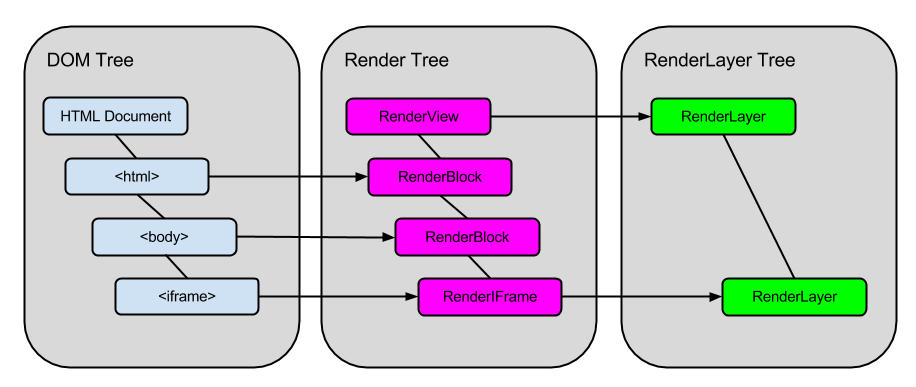
\includegraphics[scale=0.46]{rendering_trees}
    \caption{
        \label{fig-rendering-trees}
        Rendering Trees (forrás: \url{https://www.chromium.org} \cite{bib-chromium-oopifs})
    }
\end{figure}

\noindent
Az \ref{fig-rendering-trees} ábra szemlélteti, hogyan is állnak össze ezek a struktúrák.
A \texttt{DOM Tree} és a \texttt{Render Tree} szinte azonos, annyi különbséggel, hogy
a \texttt{Render Tree} csak a megjeleníthető \texttt{Node}-okat tartalmazza.
A \texttt{RenderLayer Tree} a \texttt{Render Tree} egy lecsupaszított változata, amit a
megjelenítő komponens (renderer) fog használni a rajzoláshoz.
A \texttt{RenderLayer}-ből elérhetőek a \texttt{RenderObject}-ek, a \texttt{RenderLayer Tree}
szerkezete pedig, hordozza azt az információt, hogy milyen sorrendben kell kirajzolni
\texttt{RenderObject}-eket és, hogy azok között milyen átfedések lehetnek.

Az, hogy a rajzolás hogyan történik az függ attól, hogy van e elérhető hardveres gyorsítás.
Ha nincs, akkor szoftveres renderelés történik. A szoftveres renderelés során a rajzoló
algoritmus bejárja a \texttt{RenderLayer Tree}-n keresztül a \texttt{RenderObject}-eket és
azokat egy közös bitmap-re rajzoltatja ki. Ha kész, ez a bitmap lesz elküldve egy másik
processz (browser process) számára megjelenítésre. Szoftveres renderelés esetén a rajzolást
a Skia grafikus motor végzi.

Ha van elérhető hardveres gyorsítás, akkor az eljárás valamivel bonyolultabb. Ebben az
esetben, a \texttt{RenderObject} nem bitmap-be ``rajzolja bele magát'', hanem 3D API-n
keresztül (OpenGL vagy Windows-on esetleg D3D) utasításokat küld közvetlenül a GPU
utasítás pufferébe (command buffer) végrehajtásra. Ezt az eljárást már a
Chrome Compositor (CC) végzi.
\cite{bib-chromium-gpu, bib-chromium-oopifs}

\subsection{Chrome Compositor (CC)}
A Chrome Compositor már nem része a Blink-nek (ahogy a Skia sem). Ennek az az oka,
hogy most már a Chromium a browser UI megrajzolásához is a Chrome Compositor-t használja.
Ahhoz, hogy a compositor ki tudja rajzolni a DOM-ban tárolt tartalmat, további layer
absztrakciókra van szükség:
\begin{center}
    \texttt{RenderLayers} $\rightarrow$ \texttt{GraphicsLayers} $\rightarrow$
    \texttt{WebLayers} $\rightarrow$ \texttt{CC Layers}
\end{center}

A compositor a végeredményt nem bitmap-be, hanem textúrába ``rajzolja''. Az elkészült
textúrák a GPU memóriájában vannak tárolva és úgy nevezett texture mailbox segítségével
azonosítják. A texture mailbox egy OpenGL extension kiterjesztés, ami egyedi és globális
string azonosítót rendel a textúrához és lehetővé teszi, hogy más OpenGL context-en
is elérhető legyen a textúra, ami normális esetben nem lenne megosztva.
\cite{bib-chromium-gpu, bib-chromium-oopifs}

A texture mailbox-nak hála az összeállított képet nem kell az IPC-n (Inter-Process
Communication) keresztül megosztani a processzek között (mint a szoftveres rendering
esetében), hanem a GPU memórián keresztül bármelyik processz hozzáférhet a textúrához, így
elég csak a textúra azonosítót átküldeni IPC-n.
\cite{bib-chromium-texture-mailbox}

\subsection{Multi-processz Architektúra}
Chromium volt az egyik első olyan böngésző, ami úgy lett megtervezve, hogy több processzre
legyen felosztva. A WebKit multi-processz architektúrára épülő API-ja (WebKit2) is a
Chromium-ról vette a mintát. \cite{bib-webkit-webkit2}
Ez az API a Blink-nek nem része, viszont a QtWebEngine elődjének, a QtWebKit-nek
Quick API-ja a WebKit2-re épül.

A multi-processz architektúrán alapuló böngésző alapgondolata az, hogy a böngészőalkalmazás
UI-ért felelős része saját processzben fut, míg a weboldalak megjelenítésért más
processzek felelnek. Ennek több előnye is van: \cite{bib-chromium-blog-multi-process}
\begin{description}
    \item[Felhasználói élmény]
        Előfordulhat, hogy egy weboldalon futó script (vagy ``webalkalmazás'')
        nagyon leterheli a böngészőt. Ha ez a script és a UI egy processzben fut,
        akkor ezek nagyobb valószínűséggel vonnak el egymástól erőforrást. Ha külön
        processzben, egymástól függetlenül futnak, kisebb valószínűséggel alakul ki
        köztük versenyhelyzet, így a UI nagyobb CPU használatnál is ``reszponzívabb''
        lehet.
    \item[Biztonság]
        Egyes processzek sandbox-ban futhatnak. Ezáltal nem férhetnek hozzá a rendszer
        olyan erőforrásaihoz, ami veszélyes lehet (pl. merevlemez, hálózat,
        videó memória, stb).
        Továbbá a különböző weboldalakat megjelenítő processzek egymástól is el vannak
        különítve, így egy ártalmas oldal, vagy plugin nem férhet hozzá más oldalon használt
        szenzitív információhoz (pl. jelszó).
    \item[Hibatűrés, Robosztusság]
        Ha egy oldal betöltésekor vagy egy bővítmény futtatásakor hiba történik és
        összeomlik, az nem rántja magával a teljes böngészőt. Hiba esetén a UI és más
        megnyitott oldalak, tabok megmaradnak.
    \end{description}

A multi-processz architektúrának hátrányai is vannak: ez a megoldás sokkal \\
erőforrás-igényesebb, és a megvalósítás is bonyolultabb (több hibalehetőség).
A processzek használata memória többletköltséggel jár. Továbbá, a futtatható processzek
számát limitálni kell, mert túl sok processz jelentős lassulást okozhat (pl. az ütemező
többletköltsége miatt).

A processzek IPC-n (Chromium's IPC System) keresztül kommunikálnak egymással.
A Chromium-ban 4 fő processz típust különböztetünk meg:

\subsubsection{Browser Process}
Ez az a processz, ahol maga böngésző alkalmazás (UI) fut. Ez felelős megjelenítésért,
a felhasználói események és a tabok kezeléséért. Ez a fő processz, ami a többi processzt
kezeli (indítja, leállítja, stb.) és csak egy van belőle. Hozzáfér a rendszer erőforrásaihoz,
viszont nem tölt be vagy dolgoz fel web tartalmat.

\subsubsection{Render Process}
A renderelő motor egy nagyon összetett és bonyolult szoftver komponens. Szinte lehetetlen
olyat implementálni, ami sosem hibázik és/vagy omlik össze. \cite{bib-chromium-multi-process}
Ezért racionális döntés az egymástól független oldalak renderelését egymástól független
processzekben végrehajtani. Amennyiben egy Render Process összeomlik, arról a
Browser Process értesül és az oldal helyett az \ref{fig-sad-tab} ábrán látható,
úgynevezett, ``sad tab'' értesítést jeleníti meg.

\begin{figure}[h]
    \centering
    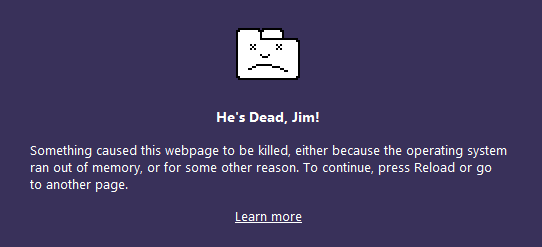
\includegraphics[scale=0.8]{sad_tab}
    \caption{
        \label{fig-sad-tab}
        Sad Tab
    }
\end{figure}

Mivel a Chromium-ban a renderelésért a Blink felel, ezért az is a Render Process-ben fut.
A Blink az, ami közvetlenül feldolgozza a webes tartalmat, ezért jellemzően a
Render Process-t sandbox-ban futtatják, így a potenciálisan kártékony webes kódok nem
férhetnek hozzá a rendszer erőforrásaihoz vagy más betöltött webes tartalomhoz.

A Chromium-ban különböző parancssori kapcsolókkal is beállítható processz modellek
vannak definiálva:
\begin{description}
    \item[Process-per-site-instance]
        Minden site\footnote{Site alatt olyan weboldalak csoportját értjük, amelyek
        közös beregisztrált domain néven osztoznak} külön processz.
        Ha ugyanaz a site kétszer van megnyitva, akkor az is két külön processz lesz.
    \item[Process-per-site]
        Különböző site-ok külön processzbe kerülnek. Az előzővel ellentétben, ha egy site
        kétszer van megnyitva, akkor azok közös processzbe kerülnek.
    \item[Process-per-tab]
        Minden tab külön processz. Több tab kerülhet közös processzbe, ha függnek egymástól.
    \item[Single Process]
        A ``hagyományos, egy-processzes'' modell. \\
        Nincs külön Render Process. A rendering a Browser Process-ben történik.
\end{description}

\noindent
Alapértelmezetten a \textit{Process-per-site-instance} modellt használja a böngésző, de
ettől függetlenül előfordulhat, hogy több site is osztozik, ugyanazon a processzen.
Erre vagy akkor van szükség amikor két site hivatkozik script-ből egymásra,
vagy amikor a futó Render Proess-ek száma elér egy limitet.
\cite{bib-chromium-process-models}

\subsubsection{Plugin Process}
A pluginok okozzák a legtöbb problémát a böngésző stabilitásának szempontjából. A plugint
egy harmadik fél készíti ezért a Chromium-nak nincs befolyása afelett, hogy milyen
erőforrásokat használ. Ennél fogva, indokolt lépés a pluginokat nem a Browser Process-ben
futtatni. A legtöbb plugin nem futhat sandbox-ban, mivel olyan
képességekkel bővítik a böngészőt, amelyekhez szükség van hozzáférésre a rendszer
erőforrásaihoz. Ezért a Render Process-en kívül szükség van egy újabb processz típusra is,
amelyben a pluginok futhatnak.
\cite{bib-chromium-plugins}

\subsubsection{GPU Process}
A renderelés a Render Process-ben történik, viszont ez a processz sandbox-ban fut és ezért
nem küldhet parancsokat GPU-nak. Hardveres gyorsítás esetén a compositing-ot és a rajzolást
egy külön processzben kell végezni, ami nem sandbox-ban fut.
\cite{bib-chromium-gpu} \\
A Chromium úgy is konfigurálható, hogy a GPU Process feladatát a Browser Process lássa el.

\subsection{Chromium Content Module}
A Content Module a Chromium az a része, ami megvalósítja az előző fejezetben bemutatott
multi-processz architektúrát. Továbbá, ebben van megvalósítva az összes támogatott
web platform funkcionalitás (például: HTML5, WebRTC, WebGL, stb.), illetve
a hardveres GPU gyorsítás. Böngészőalkalmazás specifikus funkcionalitások, nem részei
Content Module-nak. Lényegében csak az van benne, ami a web tartalom
megjelenítéséhez\footnote{\textit{content} = web tartalom} szükséges, azaz olyan kód,
amit minden böngészőt integráló alkalmazásnak szüksége van.
\cite{bib-chromium-content-module}

A modul célja, hogy az opcionális böngésző funkcionalitások (amire nem feltétlenül van
szüksége a beágyazó alkalmazásnak (pl. Chrome) le legyenek választva, ezáltal
megvalósíthatóak és testreszabhatóak legyenek a beágyazó alkalmazásban anélkül,
hogy a Chromium forráskódját módosítani kellene. Erre nyújt lehetőséget a Content API.

\subsubsection{Chromium Content API}
A Content API megtervezésekor a WebKit API-t vették alapul, hogy a WebKit fejlesztők
könnyebben áttérhessenek. Az új API \textit{unstable}, ami azt jelenti, hogy az API minden
új kiadásban változhat, ezért a beágyazó alkalmazást is minden Chromium frissítés után nagy
valószínűséggel változtatni kell.

A Content Module a beágyazó alkalmazást interfészeken (Delegate, Observer)
és callback függvényeken keresztül értesíti az eseményekről, változásokról (például,
hol tart a web oldal letöltése vagy sikeres volt-e a letöltés) vagy éppen
kér le adatokat (például, kell megjeleníteni hiba üzenetet, ha nem sikerül letölteni egy
oldalt). Az ilyen interfészek metódusainak törzse üres a Content Module-ban, ezeket a
beágyazó alkalmazásnak kell megvalósítania és a Content Module hívja meg őket szükség esetén.

Ezeken kívül vannak olyan interfészek is, amelyeket a Content Module implementál
(például, oldal betöltése: \texttt{LoadURLWithParams()} vagy az URL lekérdezése: \\
\texttt{GetVisibleURL()}).
Ezek az interfészek \textit{pure abstract} interfészek, mivel csak egy megvalósításuk lehet
és az is a Content Module-on belül. \cite{bib-chromium-content-api}

\subsubsection{Chromium Content Shell}
\begin{figure}[h]
    \centering
    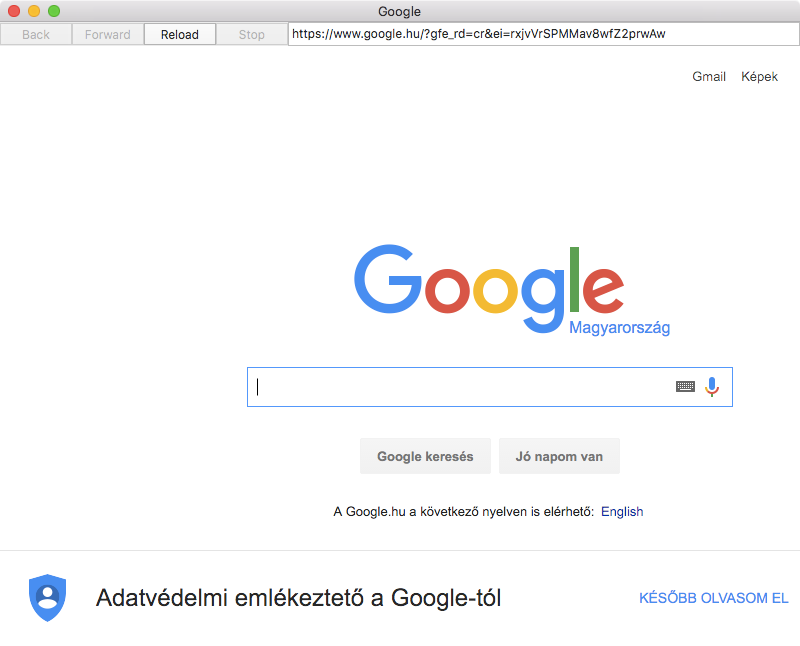
\includegraphics[scale=0.5]{content_shell}
    \caption{
        \label{fig-content-shell}
        Content Shell
    }
\end{figure}

\noindent
Az \ref{fig-content-shell} ábrán látható alkalmazás a Content Shell. Ez a lehető
legegyszerűbb böngészőalkalmazás, ami a Content API-ra épül. Arra használják, hogy a
Content Module-t és a Blink-et tesztelhessék, debuggolhassák anélkül, hogy egy teljes
böngészőalkalmazást (pl. Chrome) le kellene fordítani.

\subsection{Felépítés}
Az eddigiek alapján a Chromium-ot 3 rétegre oszthatjuk fel:
\begin{description}
    \item[Chrome]
        Felhasználói felület (UI) és böngészőalkalmazás funkciók
        (pl.: history, könyvjelzők, favicon, stb.)
    \item[Blink]
        Webes tartalom feldolgozása és renderelése. A V8 JavaScript motort a
        Blink-en keresztül érjük el és közös processzben futnak.
    \item[Content]
        Ez a réteg valósítja meg a multi-processz architektúrát,
        felel a web platform funkciókért és a hardveres GPU gyorsításért.
\end{description}
A \ref{fig-chromium-architecture} ábra mutatja, hogyan is állnak össze a Chromium rétegei.
Itt a Blink böngészőmotor még ``WebKit''-nek van jelölve.
A legfelső réteg a Chrome, helyére a saját beépítő alkalmazás kerül.

\begin{figure}[h]
    \centering
    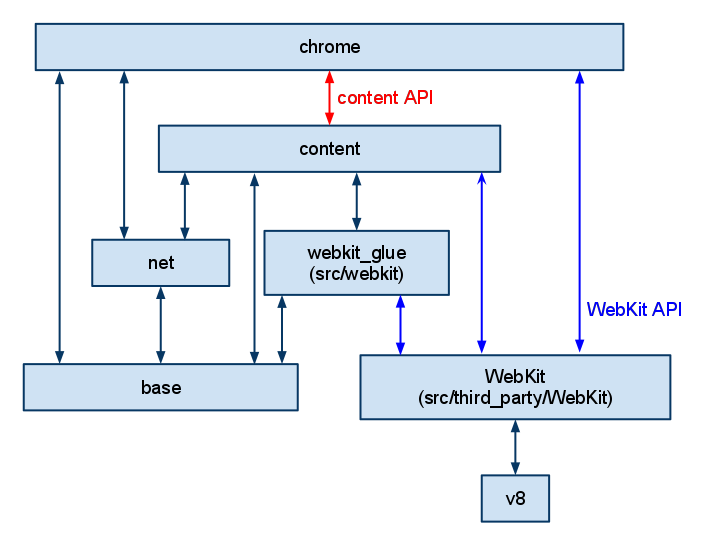
\includegraphics[scale=0.6]{chromium_architecture}
    \caption{
        \label{fig-chromium-architecture}
        Architectural Diagram
        (forrás: \url{https://www.chromium.org} \cite{bib-chromium-content-module})
    }
\end{figure}


\subsection{Chromium Release}
Egy Chromium release verzió száma 4 részből tevődik össze:
\begin{verbatim}
    MAJOR.MINOR.BUILD.PATCH
\end{verbatim}
A dolgozatomban a fő verzió számra (\texttt{MAJOR}) hivatkozok.
A Chromium közösség előre tervezett menetrend szerint 1-1.5 havonta vált fő
verziószámot. Dolgozatom készítése idején az 51-es verziójú volt a legfrissebb stabil kiadás.
Az itt leírtak erre a verzióra vonatkoznak.


\section{Qt}
A Qt egy nyílt forrású, cross-platform alkalmazás keretrendszer. Úgy ahogy a
Chromium úgy a Qt is elérhető napjaink legnépszerűbb desktop és mobil
operációs rendszerein. Ez a keretrendszer nyújt \texttt{C++} függvénykönyvtárakat (library),
binding-okat más programozási nyelvekhez (pl.: Python, Java), saját programozási nyelvet
(\texttt{QML}), saját integrált fejlesztői környezetet (QtCreator), saját build rendszert
(qmake) és kiterjesztéseket is a \texttt{C++} programozási nyelvhez (pl.: signal-slot model).
\cite{bib-qt-wiki-about-qt}

\subsection{Qt Történelem}
\subsubsection{1995-2000}
A Qt első verziója 1995-ben adta ki a Trolltech. Akkor még a projekt egy
cross-platform GUI fejlesztői keretrendszernek indult.
Nem sokkal később (1998-ban), jelent meg a
KDE (K Desktop Environment) első verziója, amely Qt-re épült.
A KDE egyhamar az egyik legnépszerűbb Linuxos asztali környezetté nőtte ki magát
és talán ennek tudható be a Qt népszerűsége is.
A Qt eszköztára az évek során fokozatosan
bővült. Új API-k jelentek meg adatbázis kezeléshez (SQL), hálózati programozáshoz,
multimédiás alkalmazások készítéséhez, XML dokumentumok feldolgozásához stb.

\subsubsection{2000-2008}
2000-ben megjelent a Qt-ra épülő Qt/Embedded keretrendszer Linux-os beágyazott eszközökre.
Ezzel az új technológiával a Qt meg is jelent az első okos telefonokon (2003: Motorola A760)
és a korabeli PDA-kon. 2006-ban a Trolltech még a saját fejlesztésű mobil telefonját is
kiadta, Greenphone néven.

\subsubsection{2008-2011}
Talán a Trolltech beágyazott platformokon és mobil telefonokon szerzett tapasztalata
miatt került arra sor, hogy 2008-ban, az akkori egyik vezető mobiltelefon gyártó, a Nokia,
felvásárolta a céget. A következő pár évben a fejlesztés még inkább a mobil eszközök
felé irányult, olyannyira, hogy azokon a részeken, melyek nem voltak érintettek mobil
fejlesztés szempontjából jóformán nem is történt fejlesztés.
2010-ben kiadott 4.7-es verzióban két nagyon fontos újítás (teljesen új modul) jelent meg:
a QtWebKit és a QtQuick.

A WebKit az Apple által fejlesztett nyílt forrású böngésző motor, a QtWebKit pedig ennek
a ``Qt portja''. Ez azt jelenti, hogy az API természetesen ``Qt-s'', továbbá a legfontosabb
``alacsony szintű'' feladatokat is a Qt látja el, mint például a hálózat kezelés
(pl. tartalom letöltése) és az oldalak kirajzolása (renderelése).
Ironikus a történetben, hogy a WebKit elődjei a KHTML és KJS projektek, melyek a KDE
keretrendszer részei voltak, ennélfogva a Qt-ra épültek. Amikor 2001-ben az Apple
fejlesztői forkolták ezeket a library-kat, a céljuk éppen az volt, hogy a Qt-tól független
böngésző motort valósítsanak meg.

A Qt 4.7-es verzió másik nagyon fontos újítása a QtQuick és a \texttt{QML}.
Ez az új technológia a mobil fejlesztés szempontjából nagyon fontos. A \texttt{QML} egy
új deklaratív programozási nyelv, a QtQuick pedig a hozzátartozó eszközkészlet vagy
``függvénykönvytár''. Ezek segítségével a Qt egy új megközelítést nyújtott GUI
megvalósítására. A legnagyobb előnye (a könnyű használhatóságot és a gyors fejlesztési
ciklust nem számítva), hogy mobil alkalmazás felhasználói felületének
lefejlesztéséhez nincs szükség szimulátorra, hiszen a \texttt{QML}-ben írt alkalmazás
platform független és ugyanúgy fut/néz ki desktop-on mint mobilon.

\subsubsection{2011-2013}
2011 elején a Nokia szerződést kötött a Microsoft-tal. A Nokia készülékek elsődleges
platformja a Windows Phone lett, így a Nokia elkezdte fokozatosan leépíteni a
szoftver kutatás-fejlesztés részlegét. 2012-re a Qt teljes egészében a Digia
tulajdonába került.

A 2012-es év más változást is hozott, az év végén megjelent a Qt 5.0-ás verziója.
Az új verzió API-ja nem sokban tér a 4-estől, ami azt jelenti, hogy az új API szinte
teljesen kompatibilis maradt. Az igazán fontos változás a Qt kód struktúrájában jelent meg.
A 4-es verzióban a kódot már modulokra bontották, hogy a Qt-s alkalmazások méretét
csökkentsék azzal, hogy a nem használt modult (gyakorlatilag library-t) nem linkelik
az alkalmazáshoz. Az 5-ös verzióban a fejlesztők tovább mentek: a keretrendszert több,
kisebb modulra bontották és az összetartozó modulokat közös repository-ba rakták
(komponensek). Ezzel megszűnt a 4-es verzió ``egy-repositorys'' modellje és így a
modulok/komponensek egymástól függetlenül is kiadhatóvá, verziózhatóvá váltak.
Az új repository-kat a \texttt{qt5} top-level repository köti össze.
Ez hivatkozásokat (git submodule) tartalmaz a modulok repository-jaira, itt találhatóak meg a
build-hez szükséges scriptek egy része és más build-hez szükséges platform specifikus fájlok
(QPA plugin-ok, mkspecs, stb.) is.

Az 5-ös verzió másik újítása QtQuick2 volt. A QtQuick első verziója (QtQuick1) a
\texttt{QGraphicsView}-ra épül, ami szoftveres renderelést használ a megjelenítéshez.
Ez a megoldás lassú, ráadásul widget függősége is van. A QtQuick2 API-ja kompatibilis a
QtQuick1-el, viszont teljesen újraírták. Nincs többé widget függőség mivel ezentúl a
QtQuick2 a \texttt{QSceneGraph}-ra épül. Ez a scene graph Open GL ES 2.0-ra vagy
Open GL 2.0-ra épül, így a renderelés a GPU-n történik. Ez a megoldás sokkal gyorsabb,
viszont nem működik olyan platformokon ahol nincs OpenGL 2.0.

2013-ban a Qt fejlesztői úgy döntenek szakítanak a WebKit-el és, hogy böngésző motor
API-jukat ezentúl a Chromium felé építik. \cite{bib-qt-blog-introducing-qtwebengine}
Az új komponenst QtWebEngine-nek hívják és 5.4-es verzióban jelent meg először.
\cite{bib-qt-wiki-qt-history}

\subsubsection{2014-napjainkig}
2014-ben a Qt részlege kivált a Digia-ból és létrejött a \textit{The Qt Company},
mint a Digia leányvállalata. A kiválás oka, hogy a Qt üzleti logikája és piaca eltér a
Digia-étól, ezért másfajta vezetésre, fejlesztésre és befektetési tervre van szükség.
Ez a folyamat még 2016-ban is tart és terv szerint 2016 májusában a The Qt Company megjelenik
a tőzsdén is.
\cite{bib-qt-about-us}

A Qt hányattatásai ellenére még ma is töretlen népszerűségnek örvend és talán az egyik
legjobb legjobb \texttt{C++} alkalmazás keretrendszer a piacon. Ezt bizonyítja,
hogy több, napjainkban is népszerű és széles körben elterjedt alkalmazás is a
Qt keretrendszerre épül. Ilyenek például a Skype, a Google Earth, a VirtualBox,
a VLC média lejátszó és a Spotify is.

\subsection{Qt Modulok és Komponensek}
A 4-es Qt verzióban megtörtént az első lépés a modularizáció felé: minden modulnak külön
library-ként jelenik meg ahelyett, hogy egy nagy közös library-je lenne a Qt-nak.
Ennek előnye, hogy a fejlesztőnek nem kell olyan modulokat az alkalmazásához linkelnie,
amit nem is használ.

Az 5-ös Qt verzióban kiterjesztették a modularizációt a projekt struktúrájára is. A projekt
többé nem egy nagy közös repository, hanem több önálló repository-ból áll össze, melyeket
a modulok szerint választottak el. Ennek előnye, hogy egyes modulok külön is release-elhetőek
(egyes modulok gyorsabban fejlődnek, mások nem), a tesztelés és buildelés rugalmasabb és
gyorsabb lett, hiszen nem kell mindig a teljes rendszert tesztelni vagy buildelni.

\begin{figure}[h]
    \centering
    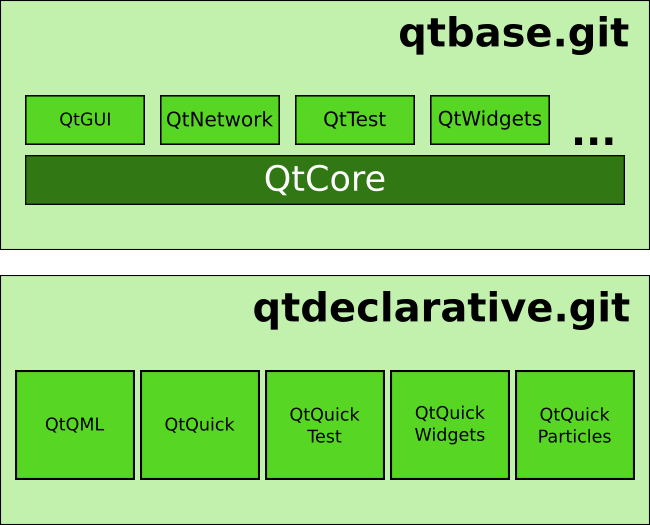
\includegraphics[scale=.66]{qt_repos_and_modules}
    \caption{
        \label{fig-qt-repos-and-modules}
        Qt repository-k és modulok
    }
\end{figure}

Továbbá, Qt 5 óta a modulokat két kategóriába sorolják: \textbf{Qt Essentials} és
\textbf{Qt Add-Ons}. A Qt Essentials-ba tartoznak azok a modulok, amelyek működnek az
összes támogatott platform-on és a legtöbb Qt alkalmazás használja is őket. Ezeknek a
moduloknak az API-ja az 5-ös verzión belül visszafele kompatibilis marad.
A Qt Add-on modulok nem általános célú, "opcionális" modulok. Vannak köztük olyanok,
amelyek nem használhatóak bizonyos Qt által támogatott platformokon vagy olyanok, amelyek
hamarosan eltávolításra kerülnek a Qt keretrendszerből, csak kompatibilitási okokból vannak
még bent (pl. QtScript). A QtWebEngine moduljai is Qt Add-On kategóriába vannak sorolva,
hiszen a legtöbb alkalmazásnak nincs szüksége böngésző funkciókra. API kompatibilitás
szabályait minden Add-On modul saját magának határozza meg.
\cite{bib-qt-doc-qtmodules}

Ha egy Qt-s alkalmazás használ egy Qt modult, akkor azt annak a projekt file-jában
(\texttt{.pro}) meg kell adni:
\begin{verbatim}
    QT += network widgets qml quick
\end{verbatim}
Ez alól kivétel a \texttt{QtCore} és a \texttt{QtGUI} modul. A \texttt{QtCore} modult
minden Qt-s alkalmazás használja, ezért azt a Qt build rendszere implicit linkeli.
Ebben a modulban vannak megvalósítva a Qt típusok és adatszerkezetek, a Qt specifikus nyelvi
elemek és makrók (pl.: \texttt{Q\_OBJECT}, \texttt{signals}, \texttt{slots}),
smart pointerek, stb. A \texttt{QtGUI} modulra a grafikus felhasználói felület
megvalósításához van szükség, de nem kötelező használni (explicit le lehet tiltani).
A \texttt{QtGUI} modulról bővebben a \ref{sec-qt-gui} fejezetben lesz szó.

Ahogy a Qt-s alkalmazások, használnak egy Qt-s modult, úgy a Qt-s modulok is használják
egymást. Az alkalmazáséhoz hasonlóan a modul projekt file-jában is meg kell adni a
függőséget. Továbbá, ha egy komponens modulja használja egy másik komponens modulját, akkor
a komponensek közötti függőséget külön jelezni kell. Erre a ``felhasználó'' komponens
\texttt{sync.profile} script-jében van lehetőség:
\begin{verbatim}
    %dependencies = (
        "qtbase" => "",
        "qtdeclarative" => "",
        "qtxmlpatterns" => "",
        "qtquickcontrols" => "",
        "qtwebchannel" => "",
    );
\end{verbatim}

\begin{figure}[h]
    \centering
    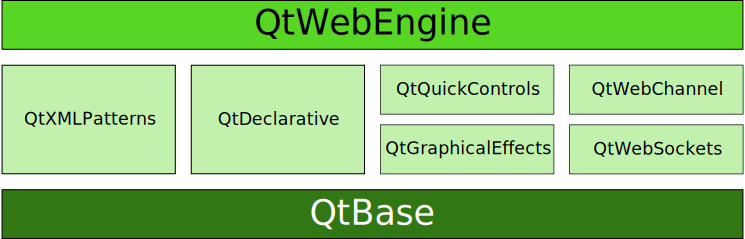
\includegraphics[scale=.66]{qtwebengine_dependencies}
    \caption{
        \label{fig-qtwebengine-dependencies}
        QtWebEngine függőségei
    }
\end{figure}

\noindent
Ebben az esetben, a komponensre, mint a modult tároló repository-ra kell
gondolni\footnote{Tovább bonyolítja a helyzetet, hogy sok esetben a komponenseket is
``modul'' elnevezéssel illetjük. Például: ``a QtWebEngine modul függősége a QtBase modul''},
ezért, ha a \texttt{QtCore} modul minden más modul függősége, értelemszerűen az őt tartalmazó
\texttt{QtBase} komponens minden más komponens függősége is lesz, amit ezen a szinten
még explicit meg kell adni.
Az \ref{fig-qtwebengine-dependencies} ábra mutatja, hogy a fenti \texttt{sync.profile} script
alapján a QtWebEngine függőségei hogyan alakulnak.


\subsection{Qt GUI}
\label{sec-qt-gui}
\begin{itemize}
    \item GUI fejlesztésre 2 API: a ``hagyományos'' Widget és a ``modern'' Quick \dots
    \item 2D: raster
    \item OpenGL integration
    \item QT -= gui
\end{itemize}

\subsubsection{Widget}
\begin{itemize}
    \item widget elemek
    \item layoutok
    \item Alkalmazás: designer
\end{itemize}

\subsubsection{Quick}
\begin{itemize}
    \item QtQuick2 OpenGL nélkül nem megy
    \item Library: Quick - Qt UI Creation Kit
    \item Declarative language: QML - Qt Modeling Language
    \item Fluid UI
    \item Logika: JavaScript
    \item QML-t is JavaScript engine dolgozza fel, jelenleg: v4
\end{itemize}

\subsection{Qt Web}
\begin{itemize}
    \item QtWebView (natív WebView, Android)
    \item QWebChannel
    \item QtWebSockets
    \item QtWebKit
    \item QtWebEngine
    \item etc.
\end{itemize}

\subsection{Qt Release}
\begin{itemize}
    \item Félévente jelennek meg új kiadások
    \item legfrissebb stabil az 5.6
    \item a dolgozatban 5.7
\end{itemize}

\section{QtWebEngine}
\begin{itemize}
    \item Qt module
    \item Unstable \texttt{Chromium Content API} felett egy stable Qt API
    \item Chromium Content Module-t beágyazó ``alkalmazás''
    \item ``Együttműködés'' (integrálhatóság) más Qt API-kal
    \item OpenGL nélkül nem megy
    \item SceneGraph
    \item Qt függőségek
        \begin{itemize}
            \item qtbase
            \item qtdeclarative
            \item \dots
        \end{itemize}
    \item Lecsupaszított \texttt{Chromium} fork is a része
\end{itemize}

\subsection{QtWebEngine Process}
\begin{itemize}
    \item Hogyan indul?
    \item Miért felel?
        \begin{itemize}
            \item Rendering
            \item etc.
        \end{itemize}
    \item IPC kommunikáció a processzek között
    \item Thread-ek
    \item Single Process mode
\end{itemize}

\subsection{QtWebEngine Core}
\begin{itemize}
    \item Mi van benne?
    \item Új (5.7): publikus API, mire jó?
    \item Design Pattern
        \begin{itemize}
            \item Delegate osztályok
            \item Adapterek
        \end{itemize}
    \item \dots
\end{itemize}

\subsection{QtWebEngine API}
\begin{itemize}
    \item D pointeres dolog (private class-ok)
    \item Bináris kompatibilitás
    \item Miért a 2 API?
    \begin{itemize}
        \item A Quick a fontosabb
        \item A 2 API között vannak funkcióbeli különbségek (``az egyik tudja, a másik nem'')
    \end{itemize}
\end{itemize}

\subsubsection{Widget}
\begin{itemize}
    \item Szinkron API -> könnyebb tesztelés
\end{itemize}

\subsubsection{Quick}
\begin{itemize}
    \item Aszinkron API -> állandó probléma a tesztelésnél
        \begin{itemize}
            \item Bizonyos események (signal-ok) bekövetkezésének a sorrendje nem garantált
        \end{itemize}
\end{itemize}

\subsection{Felépítés}
%\begin{figure}[h]
\begin{figure}[ht]
    \centering
    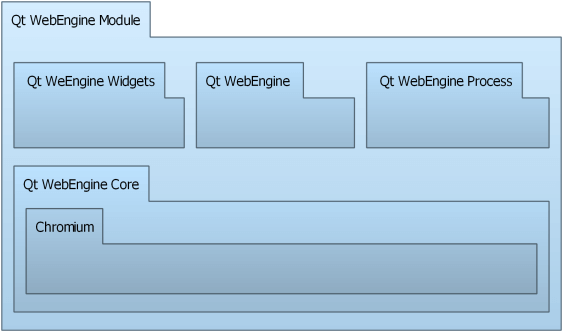
\includegraphics[scale=0.75]{qtwebengine_architecture}
    \caption{
        \label{fig-qtwebengine-architecture}
        QtWebEngine Architecture (forrás: \url{http://doc.qt.io/}
        \cite{bib-qt-doc-webengine-overview})
    }
\end{figure}


\chapter{Új funkciók a QtWebEngine-ben}

\section{Navigation History}

\begin{itemize}
    \item Hiányzó Quick API megvalósítása
    \item Backward, Forward list model
    \item TODO: Example gyártása?
\end{itemize}
\pagebreak

\section{Find Text}
\begin{itemize}
    \item Csak Quick API
    \item Tesztek portolása QtWebKit-ből
\end{itemize}
\pagebreak

\section{Log Level}
\begin{itemize}
    \item Parancssori kapcsoló
    \item Hibakeresés
    \item \texttt{-{}-log-level}
\end{itemize}
\pagebreak

\section{Test Support API}
\begin{itemize}
    \item Olyan feature-ök tesztelése ami nem jelenhet meg a publikus API-ban
    \item Pl. error page, az error page signal-okat elrejtjük a fejlesztő elől, de tesztelni
        kell.
    \item Előfordulhat, hogy a fejlesztő saját felelőségére használja
    \item Nincs dokumentálva
    \item Fontos lépés a tesztelés szempontjából
    \item Experimental API eltávolítása
\end{itemize}
\pagebreak

\section{Form Validation}
\begin{itemize}
    \item kódnév: Bubi
    \item Message Bubble
    \item HTML5 feature
    \item Chromium callback megvalósítása
    \item Quick és Widget API-ban kétféleképpen megrajzolt buborék
    \item Test Support API teszt
\end{itemize}
\pagebreak

\section{Localization}
\begin{itemize}
    \item Tesztelés miatt: csak angol nyelvű hibaüzenetek
    \item Qt API-n keresztül beállított lokalizáció használata
    \item \texttt{-{}-lang} parancssori kapcsoló lokalizáció felüldefiniálására
    \item \texttt{Chromium} specifikus
\end{itemize}
\pagebreak

\section{Authentication Dialog}
\begin{itemize}
    \item Dialog Quick-hez: \texttt{AuthenticationDialogController}
    \item HTTP authentication
        \begin{itemize}
            \item Simple authentication
            \item Kerberos?
        \end{itemize}
    \item Proxy authentication
    \item Jelszóval védett oldalak esetén dobjon fel ablakot a felhasználó név és jelszó
        megadásához
        \begin{itemize}
            \item pl. \url{wiki.sed.hu}
        \end{itemize}
    \item Probléma, authentikált oldalak esetén nem lehet letölteni a favicon-t
        \begin{itemize}
            \item Widget: QNAM (QNetworkAccessManager) tölti le az ikont, viszont nem kapja
                meg a bejelentkezéshez szükséges credentials-t
            \item Quick: Image QML elem van használva a kép megjelenítésére (ikon támogatás a
                QML-ben nincs).
            \item Az Image QML elem implicit elvégzi a letöltést, ami a felhasználó elől
                rejtve marad => nincs lehetőség authentikációra
        \end{itemize}
    \item Empty credentials és cancel
\end{itemize}
\pagebreak

\section{Favicon Manager}
\begin{itemize}
    \item Ikonok letöltése a Chromium Content API-n keresztül
    \item Az összes ikon letöltése és a legjobb minőségű propagálása
        \begin{itemize}
            \item Az eredeti megvalósításban a touch ikonok nem voltak kezelve
            \item Fontos lehet érintő kijelzős eszközökön vagy akár desktop gépeken is
            \item A history vagy könyvjelzők megjelenítés nagy méretű ikonokkal
        \end{itemize}
    \item Konfigurálhatóság a WebEngineSettings-en keresztül (``Icon Download Modes'')
        \begin{itemize}
            \item Letilthatóak lehessenek az ikonok (sávszélesség, sebesség, saját icon
                manager)
            \item Desktop-on alapból nincsenek bekapcsolva a touch ikonok, de engedélyezni
                lehessen őket
        \end{itemize}
    \item Terv: egy QIcon-ban ``összegyúrva'' az összes ikon
        \begin{itemize}
            \item a felhasználó extra API nélkül könnyedén kiválaszthatja a számára
                megfelelő méretet
            \item Quick esetében az Image átméretezésekor a megfelelő felbontású ikon
                kerül betöltésre
        \end{itemize}
    \item widget API-ra példa QtWebKit-ből
        \begin{itemize}
            \item Azért van szükség módosításra
            \item kész dokumentáció
        \end{itemize}
    \item Quick API-hoz icon image provider
        \begin{itemize}
            \item problémák: hogyan kössük be a manager-t? Hol kössük be a provider-t az
                engine-be?
        \end{itemize}
    \item Hosszabb távú tervek (Qt 5.8)
        \begin{itemize}
            \item API bővítése az elérhető ikonok listázására és explicit letöltésére
            \item Icon database: merevlemezen tárolt ikonok (oldal betöltése előtt is
                elérhető legyen vagy offline módban)
        \end{itemize}
\end{itemize}
\pagebreak


\chapter{Egy példa böngészőalkalmazás megvalósítása}
\textbf{Szempontok:}
\begin{itemize}
    \item Screenshot-ok legyenek a browser-ről
    \item Csak a lényeget részletezni (funkciók megjelenése), a ``körítés'', design-t csak
        megemlíteni
    \item QML példakód a funkciókra
\end{itemize}

\noindent
\textbf{Gondolatok:}
\begin{itemize}
    \item Gyors billentyűre felugró pop-up, amibe az URL-t lehet írni. Animált (halványodik),
        félig áttetsző
    \item Az URL pop-up-nak legyen saját history-ja a memóriában (csak addig él amíg a
        program fut). Indításkor a navigation history-ból legyen inicializálva.
        Automatikus URL kiegészítés.
    \item Legyenek az oldalakról screenshot-ok tárolva. Az URL pop-up a felajánlott oldalakkal
        együtt mutatja a screenshot-ot.
    \item A tabok bal oldali sávon legyenek, vertikális listában. Indok: desktop browser,
        a monitorok szélesek
    \item A tab bar-hoz nem használható a Quick TabView
    \item Tab bar-nak 3 állapota megjelenés szerint:
        \begin{description}
            \item[hidden] Rejtett mód
            \item[compact] ``Keskeny'' mód. Csak ikon, vagy ikon és alatta a title.
            \item[full] A tab teljes szélességében
        \end{description}
    \item Módok között a váltás animált
    \item Jobb oldalt Bookmark Bar hasonló módokkal mint a Tab Bar
    \item A Bookmark Bar-on a legfelső ikon/bejegyzés a menü
    \item Menü dialog-ok animálva jelennek meg, amely mögött a \texttt{WebEngineView}
        megváltozik. Például, összemegy, elhalványul, mindkettő, stb.
    \item Tab váltáskor az aktuális WebEngineView animálva kiúszik a képernyőről és az
        új beúszik (slide?)
    \item A tabok rendezhetőek lehessenek a Tab bar-on.
    \item A tabok csoportokba rendezhetőek legyenek.
    \item A tab felett pár másodpercig tartott egérkurzor preview-t jelenít meg a \\
        \texttt{WebEngineView}-ról
    \item Egyedi dialog ablakok, ha addig elkészül a custom UI delegate
\end{itemize}

\noindent
\textbf{Funkciók megjelenése a példa browserben:}
\begin{description}
    \item[Navigation History] Legyen külön ``navigator'' ablak. Listában lépkedek az
        elemeken, kicsinyített nézetben látszik az oldal (esetleg screenshot?). Klikk-re
        kilép a navigátorból és megnyitja az oldalt.
    \item[Find Text] Ctrl+f shortcut -> animált pop-up. Regexet be lehetne-e adni?
    \item[Log Level] Példa browser indításakor \texttt{-{}-log-level} kapcsolóval
    \item[Test Support API] --
    \item[Form Validation] Screenshot a buborékról
    \item[Localization] Példa browser indításakor \texttt{-{}-lang} kapcsolóval
    \item[Authentication Dialog] Felül definiálni Custom UI delegate-el ha meg lesz
    \item[Favicon Manager] Nagy méretű ikonok: tab, bookmark (kompakt mód), URL pop-up
\end{description}

\addtocontents{toc}{\ }
\chapter*{Eredmények}
\addcontentsline{toc}{section}{Eredmények}
\begin{itemize}
    \item Eredmények:
        \begin{itemize}
            \item Hány darab új feature? Milyen kategória (QtWebKit, Test/Debug, HTML5)?
            \item Teszt lefedettség?
            \item Hány db patch ment be? Melyik milyen jellegű?
                \begin{itemize}
                    \item Új feature
                    \item Új teszt
                    \item Bug fix, build fix, teszt javítás
                    \item Chromium fork karbantartás
                    \item \dots
                \end{itemize}
            \item Chromium fork külön repository, oda is mentek patch-ek
            \item Javításaim között vannak olyanok, amelyek kimondottan platform specifikus
                problémát javítanak. Ezek lefedik a 3 fő desktop platformot: GNU/Linux,
                Windows, OS X
        \end{itemize}
    \item Összegzés?
        \begin{itemize}
            \item Hol tartunk most a QtWebKit leváltással? Mi hiányzik még?
            \item Jelenleg Qt 5.7-en dolgozunk, a felsorolásból mely feature-ök kerülnek
                be az 5.7-be: \textbf{favicon}
            \item Jövő: milyen tervek vannak 5.8-ra?
        \end{itemize}
\end{itemize}


%%% EPILOGUE %%%

\begin{thebibliography}{9}
    \addcontentsline{toc}{section}{Irodalomjegyzék}

    \bibitem{bib-qt-blog-introducing-qtwebengine}
        Qt Blog: Introducing the Qt WebEngine \\
        \href{http://blog.qt.io/blog/2013/09/12/introducing-the-qt-webengine/}
        {http://blog.qt.io/blog/2013/09/12/\\
        introducing-the-qt-webengine/}

    \bibitem{bib-wiki-chromium}
        Wikipedia: Chromium (web browser) \\
        \url{https://en.wikipedia.org/wiki/Chromium_(web_browser)}

    \bibitem{bib-wiki-chrome}
        Wikipedia: Google Chrome \\
        \url{https://en.wikipedia.org/wiki/Google_Chrome}

    \bibitem{bib-wiki-blink}
        Wikipedia: Blink (web engine) \\
        \url{https://en.wikipedia.org/wiki/Blink_(web_engine)}

    \bibitem{bib-chromium-displays-web-pages}
        Chromium: How Chromium Displays Web Pages \\
        \href{https://www.chromium.org/developers/design-documents/displaying-a-web-page-in-chrome}
        {https://www.chromium.org/developers/design-documents/\\
         displaying-a-web-page-in-chrome}

    \bibitem{bib-chromium-blink}
        Chromium: Blink \\
        \url{http://www.chromium.org/blink}

    \bibitem{bib-chromium-gpu}
        Chromium: GPU Accelerated Compositing in Chrome \\
        \href{https://www.chromium.org/developers/design-documents/gpu-accelerated-compositing-in-chrome}
        {https://www.chromium.org/developers/design-documents/\\
        gpu-accelerated-compositing-in-chrome}

    \bibitem{bib-chromium-oopifs}
        Chromium: Rendering and compositing out of process iframes \\
        \href{https://www.chromium.org/developers/design-documents/oop-iframes/oop-iframes-rendering}
        {https://www.chromium.org/developers/design-documents/\\
        oop-iframes/oop-iframes-rendering}

    \bibitem{bib-chromium-texture-mailbox}
        Chromium: CHROMIUM\_texture\_mailbox.txt \\
        \href{https://src.chromium.org/viewvc/chrome/trunk/src/gpu/GLES2/extensions/CHROMIUM/CHROMIUM_texture_mailbox.txt}
        {https://src.chromium.org/viewvc/chrome/trunk/src/gpu/\\
        GLES2/extensions/CHROMIUM/CHROMIUM\_texture\_mailbox.txt}

    \bibitem{bib-webkit-webkit2}
        WebKit: WebKit2 \\
        \url{https://trac.webkit.org/wiki/WebKit2}

    \bibitem{bib-chromium-multi-process}
        Chromium: Multi-process Architecture \\
        \href{https://www.chromium.org/developers/design-documents/multi-process-architecture}
        {https://www.chromium.org/developers/design-documents/\\
        multi-process-architecture}

    \bibitem{bib-chromium-blog-multi-process}
        Chromium Blog: Multi-process Architecture \\
        \href{http://blog.chromium.org/2008/09/multi-process-architecture.html}
        {http://blog.chromium.org/2008/09/\\
        multi-process-architecture.html}

    \bibitem{bib-chromium-process-models}
        Chromium: Process Models \\
        \href{https://www.chromium.org/developers/design-documents/process-models}
        {https://www.chromium.org/developers/design-documents/\\
        process-models}

    \bibitem{bib-chromium-plugins}
        Chromium: Plugin Architecture \\
        \href{https://www.chromium.org/developers/design-documents/plugin-architecture}
        {https://www.chromium.org/developers/design-documents/\\
        plugin-architecture}

    \bibitem{bib-chromium-content-module}
        Chromium: Content module \\
        \url{https://www.chromium.org/developers/content-module}

    \bibitem{bib-chromium-content-api}
        Chromium: Content API \\
        \href{https://www.chromium.org/developers/content-module/content-api}
        {https://www.chromium.org/developers/content-module/\\
        content-api}

    \bibitem{bib-qt-wiki-about-qt}
        Qt Wiki: About Qt \\
        \url{https://wiki.qt.io/About_Qt}

    \bibitem{bib-qt-wiki-qt-history}
        Qt Wiki: Qt History \\
        \url{https://wiki.qt.io/Qt_History}

    \bibitem{bib-qt-doc-webengine-overview}
        Qt Documentation: Qt WebEngine Overview \\
        \url{http://doc.qt.io/qt-5/qtwebengine-overview.html}

    \bibitem{bib-qt-about-us}
        The Qt Company: About Us \\
        \url{http://www.qt.io/about-us}

    \bibitem{bib-qt-doc-qtmodules}
        Qt Documentation: All Modules \\
        \url{http://doc.qt.io/qt-5/qtmodules.html}

\end{thebibliography}


\chapter*{Nyilatkozat}
\addcontentsline{toc}{section}{Nyilatkozat}

\noindent
Alulírott Varga Péter programtervező informatikus MSc szakos hallgató, kijelentem, hogy a
dolgozatomat a Szegedi Tudományegyetem, Informatikai Tanszékcsoport Szoftverfejlesztés
Tanszékén készítettem, programtervező informatikus MSc diploma megszerzése érdekében.

Kijelentem, hogy a dolgozatot más szakon korábban nem védtem meg, saját munkám eredménye
és csak hivatkozott forrásokat (szakirodalom eszközök, stb.) használtam fel.

Tudomásul veszem, hogy a diplomamunkámat a Szegedi Tudományegyetem Informatikai Tanszékcsoport
könyvtárában, a helyben olvasható könyvek között helyezik el.

\vspace*{2cm}

\begin{tabular}{lc}
    Szeged, \today \hspace{2cm} & \makebox[6cm]{\dotfill} \\
                                & aláírás
\end{tabular}


\chapter*{Köszönetnyílvánítás}
\addcontentsline{toc}{section}{Köszönetnyílvánítás}

\noindent
Szeretnék köszönetet mondani Dr. Kiss Ákos témavezetőmnek a téma kutatása alatt nyújtott
támogatásáért és a diplomamunkám megírásában nyújtott segítségéért.

Ezen kívül szeretnék köszönetet mondani a \textit{The Qt Company} és a
\textit{Szegedi Tudományegyetem Szoftverfejlesztés Tanszék} volt es jelenleg is a QtWebEngine
projekten dolgozó munkatársainak a beszélgetésekért és a közösségnek benyújtott munkám
ellenőrzéséért és befogadásáért.


\chapter*{Mellékletek}
\addcontentsline{toc}{section}{Mellékletek}

\noindent
DVD lemez mely tartalmazza:
\begin{itemize}
    \item \texttt{QtWebEngine} modul \texttt{Git} repository-ját
    \item A bemutatott funkciókat megvalósító patch-eket
    \item A példa böngészőalkalmazás forráskódját
\end{itemize}

\end{document}
